%% The lines that are not written within % .. % are not to be tampered with!!

\documentclass[twoside]{article}
\setlength{\oddsidemargin}{0.25 in}
\setlength{\evensidemargin}{-0.25 in}
\setlength{\topmargin}{-0.6 in}
\setlength{\textwidth}{6.5 in}
\setlength{\textheight}{8.5 in}
\setlength{\headsep}{0.75 in}
\setlength{\parindent}{0 in}
\setlength{\parskip}{0.1 in}

%
% ADD PACKAGES here:
%

\usepackage{amsmath,amsfonts,graphicx,amsthm,amssymb}
\usepackage{subfig}

\newcounter{lecnum}
\renewcommand{\thepage}{\thelecnum-\arabic{page}}
\renewcommand{\thesection}{\thelecnum.\arabic{section}}
\renewcommand{\theequation}{\thelecnum.\arabic{equation}}
\renewcommand{\thefigure}{\thelecnum.\arabic{figure}}
\renewcommand{\thetable}{\thelecnum.\arabic{table}}


\newcommand{\lecture}[4]{
   \pagestyle{myheadings}
   \thispagestyle{plain}
   \newpage
   \setcounter{lecnum}{#1}
   \setcounter{page}{1}
   \noindent
   \begin{center}
   \framebox{
      \vbox{\vspace{2mm}
    \hbox to 6.28in { {\bf SC 607: Optimization
		\hfill Spring 2019} }
       \vspace{4mm}
       \hbox to 6.28in { {\Large \hfill Lecture #1: #2  \hfill} }
       \vspace{2mm}
       \hbox to 6.28in { {\it Instructor: #3 \hfill Scribes: #4} }
      \vspace{2mm}}
   }
   \end{center}
   \markboth{Lecture #1: #2}{Lecture #1: #2}

   {\bf Note}: {\it LaTeX template courtesy of UC Berkeley EECS dept.}

   {\bf Disclaimer}: {\it These notes have not been subjected to the
   usual scrutiny reserved for formal publications.  They may be distributed
   outside this class only with the permission of the Instructor.}
   \vspace*{4mm}
}



\renewcommand{\cite}[1]{[#1]}
\def\beginrefs{\begin{list}%
        {[\arabic{equation}]}{\usecounter{equation}
         \setlength{\leftmargin}{2.0truecm}\setlength{\labelsep}{0.4truecm}%
         \setlength{\labelwidth}{1.6truecm}}}
\def\endrefs{\end{list}}
\def\bibentry#1{\item[\hbox{[#1]}]}

%Use this command for a figure; it puts a figure in wherever you want it.
%usage: \fig{NUMBER}{SPACE-IN-INCHES}{CAPTION}
%This is for your help while typing the notes
\newcommand{\fig}[3]{
			\vspace{#2}
			\begin{center}
			Figure \thelecnum.#1:~#3
			\end{center}
	}
% Use these for theorems, lemmas, proofs, etc. 
% See how they are used, below 
\newtheorem{theorem}{Theorem}[lecnum]
\newtheorem{lemma}[theorem]{Lemma}
\newtheorem*{remark}{Remarks}
\newtheorem{define}{Definintion}[lecnum]

\newcommand\E{\mathbb{E}}
\DeclareMathOperator*{\minimize}{minimize}

\begin{document}

\lecture{15}{March 8 2019}{Ankur A. Kulkarni}{Arun Kumar Miryala, Anuraag Tummanapally}%In place of scribe-name, write down your names or your group names

\section{Review}
In the previous lecture, a necessary and sufficient condition for $x^{*}$ to be a minimizer for convex optimization problem was derived. A condition on local minimizer $x^{*}$, where $x^{*}$ is constrained over the tangent cone set $T(x^{*}, S)$,  $S$ need not be convex is found. Let us recall some of the concepts that were discussed.
\begin{theorem}
Let $S$ be a convex set and let $f$ be a continuously differentiable ($C^{1}$) convex function. Consider the following convex optimization problem:


\begin{align}
    \displaystyle{\minimize_{\text{subject to }x\in S} f(x)}
\end{align}
Then $x^{*}$ is minimizer if and only if $\:\nabla f(x^{*})^\top(y-x^{*}) \geqslant 0$, for all $y\in S$.
\end{theorem}
\begin{define}
For $x^{*} \in S$, the tangent cone $T(x^{*};S)$ is defined as:
\begin{equation}\label{eq6}
T(x^{*},S) := \bigg\{d\;\bigg|\; \exists\;{x_{k}}\subseteq S: {x_{k}}\rightarrow x^{*} \; \& \; t_k\downarrow 0\;s.t.\;d=\lim_{k \to \inf} \frac{x_k-x^{*}}{t_k}\bigg\}.
\end{equation}
Tangent cone of a set captures the precise shape of the set.
\end{define}

Example: 

In Fig \ref{fig:example}a, the tangent cone is just a straight line,and in Fig \ref{fig:example}b, the tangent cone at $x$ is entire $\mathbb{R}^2$

If $x \in \overset{o}{S}$, T(x,S) = $\mathbb{R}^2$
\begin{figure}[h]
%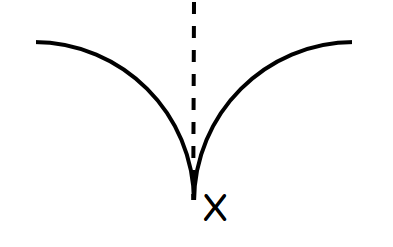
\includegraphics[scale=0.5]{images/pic1.png}
	\centering
    \subfloat[]{{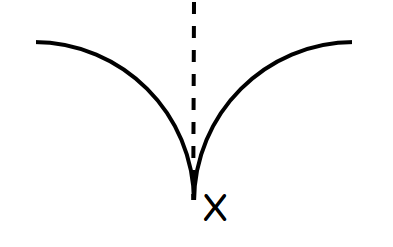
\includegraphics[width=5cm]{images/pic1.png} }}
    \qquad
    \subfloat[]{{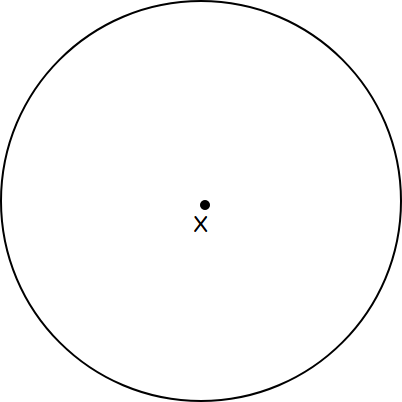
\includegraphics[width=5cm]{images/pic2.png} }}
    \caption{Tangent cone examples}
    \label{fig:example}
\end{figure}

\begin{theorem}
Consider the optimization problem:
\begin{center}
    $\displaystyle{\minimize_{\text{subject to }x\in S} f(x)}$
\end{center}
where $f \in C^{1}$. If $x^{*}$ is a local minimum, then $\nabla f(x^{*})^{\top}d \geqslant 0, \hspace{1mm}\forall d \in T(x^{*},S).$
\end{theorem}



\section{Introduction}
In this lecture, Constraint Qualifications are discussed. Farkas Lemma and Karush kuhn Tucker conditions for an optimisation problem with inequality constraints are proved  

\section{Motivation for need of Constraint Qualification(CQ)}
From Theorem 15.1 local minima $x^*$ satifies the condition $\nabla f(x^{*})^{\top}d \geqslant 0, \hspace{1mm}\forall d \in T(x^{*},S).$ for $f \in C^{1}$ and $x \in S$

here d is from Tangent Cone, When the set is convex the Tangent Cone contains all the directions including limiting direction which grazes the boundary (we cannot move further in that direction) of the set.\\
So, for any $y \in S$ entire $ y-x^*$ segment will be in the Tangent Cone \\

$$\:\nabla f(x^{*})^\top(y-x^{*}) \in T(x^{*},S)  \; \forall \;y\in S \iff x^* \text{ is a global minimum}$$

\begin{figure}[h]
\center
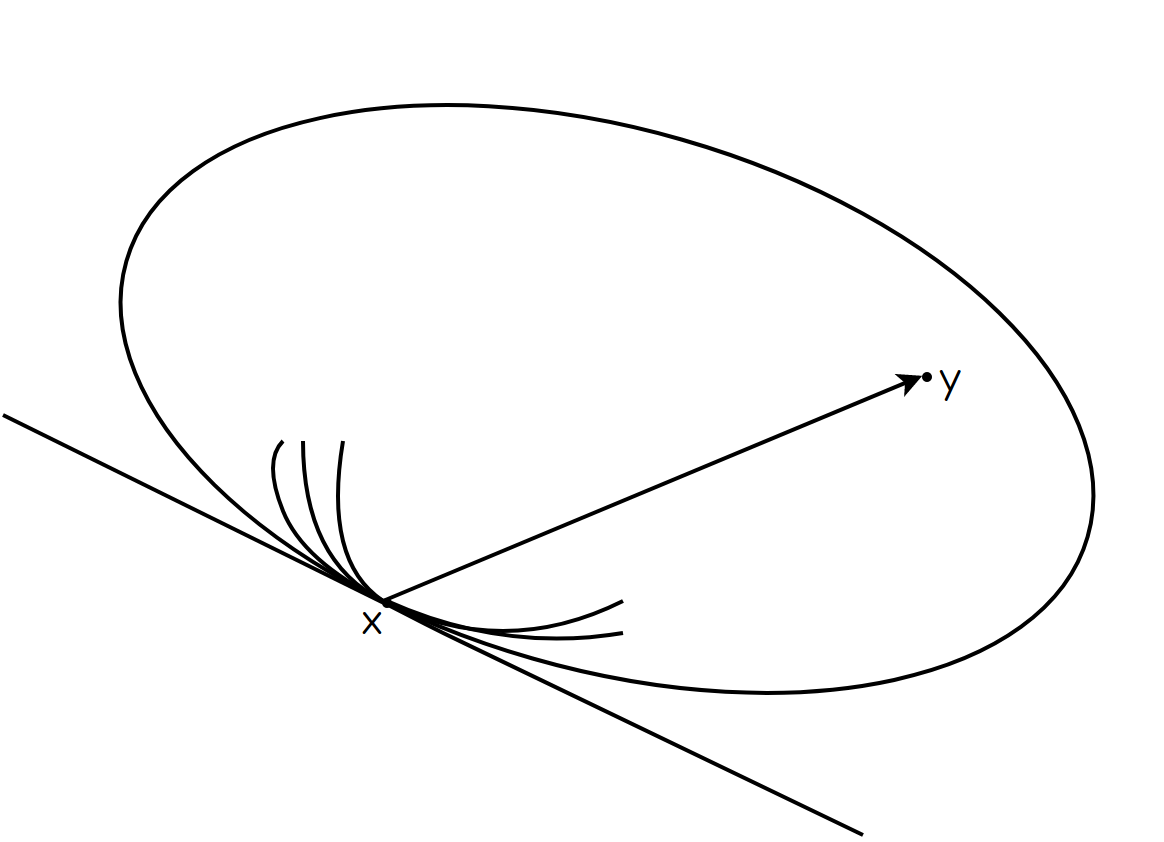
\includegraphics[width=10cm]{images/pic3.png}
\caption{$(y-x^*) \in T(X^*, S)$ when S is convex}
\end{figure}

when the set is convex necessary condition for existance of local minima will be sufficient for finding the global minima.\\

\subsubsection{Finding Tangent Cone}

Consider a optimisation problem 
\begin{center}
    Minimize $f(x)$\\
    subject to $ g(x) = x^{2}_{1}+x^{2}_2-r^{2}$\\$x\geq0$ 
\end{center}

\begin{figure}[h]
\center
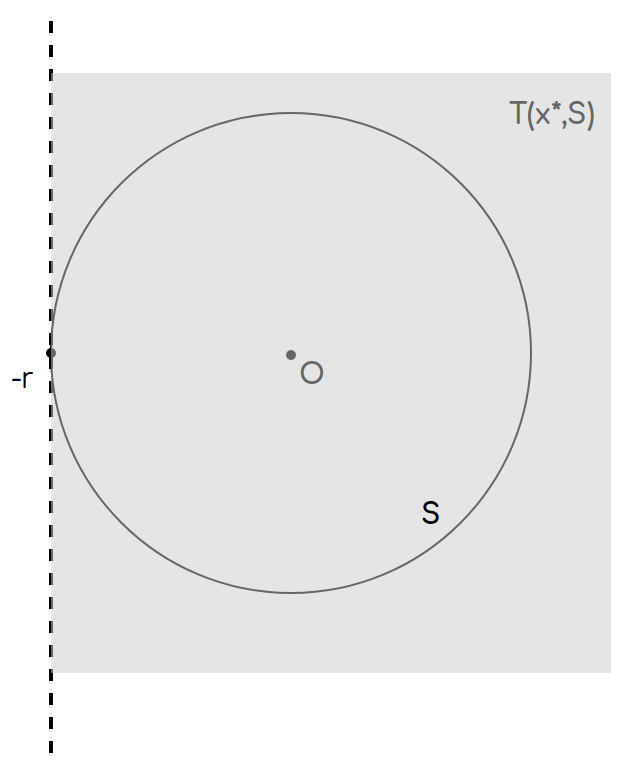
\includegraphics[scale=0.35]{images/pic4.png}
\end{figure}

Tangent cone is given by 
$\{\,d\mid \nabla g(x^*)^\mathsf{T}d\leq 0 \}$

If $x^{*}$ is in interior of the set then tangent cone is entire space $\mathbb{R}^n$\\

In the above case there was only one constraint so it is easy obtain the tangent cone. Consider the following optimisation problem 
\begin{center}
	minimize $f(x)$\\
	subject to $$S = \{\,x\mid g_{i}(x)\leq 0 , i = 1,2,...m\}$$
\end{center}

\begin{figure}[h]
\center
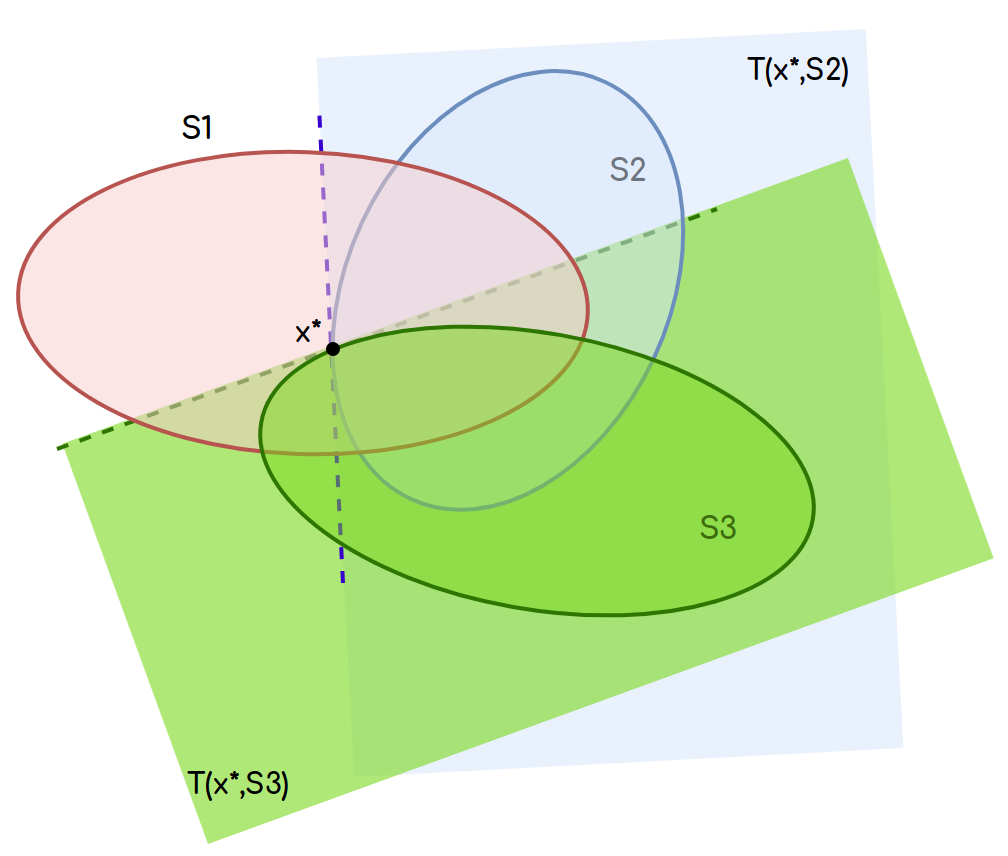
\includegraphics[scale=0.25]{images/pic5.png}
\end{figure}
let $$S = \cap^{m}_{i=1}S_i$$ where $$S_i = \{ x\mid g_i(x)\leq 0\}$$
we want $T(x^*:S)$ and we have $T(x^*:S_i)$
we can say $$T(x^*:S) \subseteq \cap_{i=1}^{m}T(x:S_i)$$
$$T(x^*:S)\nsupseteq \cap_{i=1}^{m}T(x:S_i)$$

suppose 
\begin{center}
minimize $f(x)$\\
subject to $$S = \{\,x\mid g_{i}(x)\leq 0 , i = 1,2,...m\}$$\\
$h_j(x) = 0, , j = 1,2,...p$
\end{center}

\begin{figure}[h]
\center
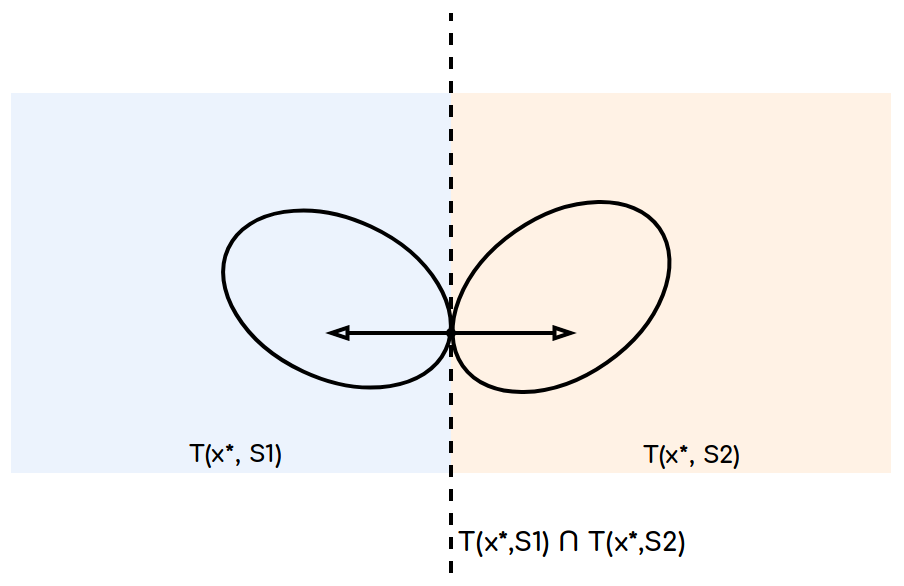
\includegraphics[scale=0.25]{images/pic6.png}
\end{figure}

\begin{figure}[h]
\center
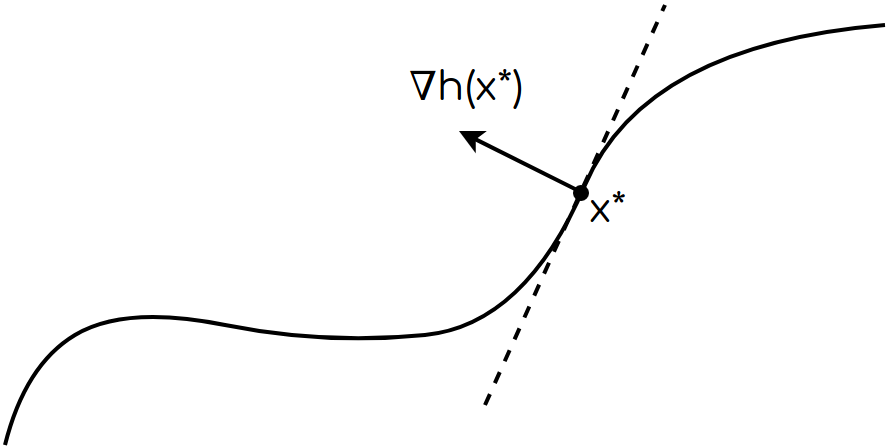
\includegraphics[scale=0.25]{images/pic7.png}
\end{figure}

same equality constraints can be represented as $\{ x \mid h^{2}_{j}(x) = 0\}$ in such representation $\nabla h_j(x)$ does not give true normal. This might happen because of Linear Dependency of Normals. Constraints Qualification makes sure that normals are linearly independent.



\subsection{Constraint Qualification (CQ)}
Let $S = \{\,x\mid g_{i}(x)\leq 0 , i = 1,2,...m\},g \in C^{1}  $ we say that a constraint qualification is satisfied at $x^{*}\in S$ if 

$$ T(x^{*},S) = \{d \mid \nabla g_i(x^*)^Td \leq 0\, \forall\, i \in I(x^*)\}$$

active constraints are such that 
$I(x^*)=\{i\mid g_i(x^*)=0\}$
for other constraints $T(x^*:S)= \mathbb{R}^n$

\section{Farkas Lemma}
\begin{lemma}
Let $A\in\mathbb{R}^{m x n}, c\in \mathbb{R}^{n}$ Then the following statements are equivalent \\
(1) $\forall x \in \mathbb{R}^{n} \text{such that }Ax \leq 0 $, we have $c^{T}x\leq 0 $\\
(2) $ \exists \, \lambda \geq 0 \in \mathbb{R}^{m}$ such that $A^{T}\lambda = C $ 
\end{lemma}
\begin{proof}
	consider  $$max c^{T}x $$ $$ \text{subject to } Ax \leq 0$$ Dual of this can be given as $$min 0 $$ $$ \text{subject to }A^{T}\lambda = c$$  $$\text{           }\lambda \geq 0$$

(1) implies optimal value of primal is $0$ which again, implies dual is feasible which implies (2)\\
(2) implies dual is feasible which inturn implies optimal value of dual is 0 which means primal is feasible there by optimal value of primal is 0 which implies (1)\\
\end{proof}


\section{Karush-kuhn-Tucker Conditions}
\begin{theorem}
Consider the problem $f,\,g_1,...,g_m \in C^{1}$ 
$$max f(x) $$
$$ g_i(x) \leq 0 \, i=1,...,m $$
Let $x^*$ be a local maximum and suppose that Constraint Qualification is satisfied at $x^*$. Then $ \exists \, \lambda_1^*,\lambda_2^*,...,\lambda_m^* \geq 0 $ such that \begin{equation}
\nabla f(x^*) = \sum_{n=1}^{m} \lambda_i^* \nabla g_i(x^*)
\end{equation}
\begin{equation}
\lambda_i^*g_i(x^*) = 0 \ \forall i = 1,2,...,m 
\end{equation}
 $  \lambda_1^*,\lambda_2^*,...,\lambda_m^* $ are Lagrange multipliers
\end{theorem}
\begin{proof}
$x^* $ is a local maxima\\
$$\nabla f(x^*)^{T}d \leq 0\, \forall \  d\in T(x^*:S)$$
but since CQ holds at $x^*$
$$T(x^*:S) = \{ d \mid \nabla g_i(x^*)^{T}d \leq 0\  \forall\  i \in I(x^*)\}$$
By Farkas Lemma $\exists \lambda_j, j \in I(x^*),\lambda_j \geq 0 $ such that $\nabla f(x^*) = \sum_{j\in I(x^*)} \lambda_j^* \nabla g_i(x^*)$\\
$$ =\sum_{j=1}^m \lambda_j^* \nabla g_i(x^*)\text{ and }\lambda_j^* = 0 , j\notin I(x^*)$$.
\end{proof}

This conditions are further generalised when equality constraints are added along with inequality constraints in next lecture.
%\section*{References}

\end{document}